В целях автоматизации процесса формирования конфигураций для модулей \texttt{remap} велась разработка соответствующего программного обеспечения. Первым делом в ручном режиме была изучена структура входных данных и сформирован профиль переупорядоченных данных выходного интерфейса. Для каждого участка жидкоаргонового калориметра существует карта, согласно которой оцифрованные значения АЦП поступают в сигнальный процессор LASP. Они представлена в виде таблиц, каждая из которых состоит из 88 строк и 6 колонок, в соответствии с количеством подключаемых входных каналов и временных ячеек для передачи данных в рамках каждого канала. Каждая ячейка содержит аббревиатуру, несущую в себе полную информацию об источнике сигнала. Поскольку калориметры имеют некоторую регулярность в своей структуре, то из всех четырёхсот карт можно выделить всего двадцать уникальных, в которых структура входных данных является действительно уникальной. То есть достаточно составить двадцать схем перестановок, и применить одну из них для каждой из существующих. Пример карты упорядочивания входных значений для участка цилиндрической части жидкоаргонового калориметра изображен на рисунке \ref{fig:remap_remapping}. При составлении выходной карты данных в первую очередь преследовалось удобное расположение данных для последующего вычисления сумм по участкам калориметра.\par
\begin{figure}[ht]
    \centering
    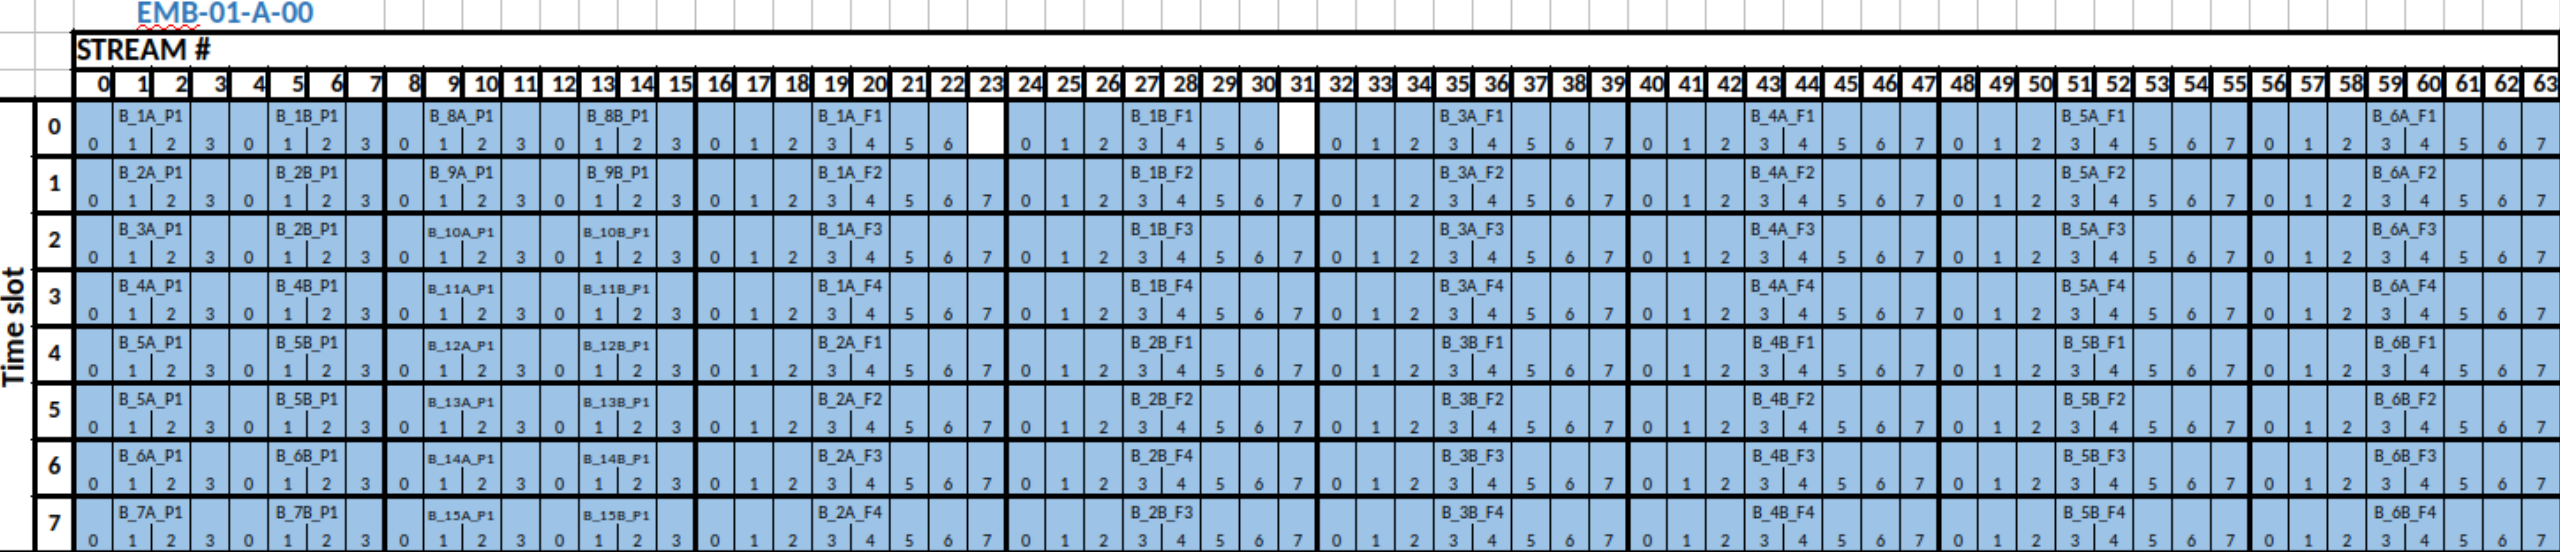
\includegraphics[width=\linewidth]{remap_remapping.png}
    \caption{Пример схема упорядочивания выходных данных модуля remap}
    \label{fig:remap_remapping}
\end{figure}\par
С помощью скрипта написанного на языке Python выполняется автоматическая генерация конфигурационных значений для модуля \texttt{remap}. Первый этап его работы заключается в подборе такого порядка значений внутри каждого отдельного входного канала, который обеспечивал бы отсутствие пересечений данных, предназначенных для каждого выходного канала, по временным ячейкам. Эти перестановки предназначаются для реализации модулем \texttt{ialign}. Следующим этапом является поиск последовательности номеров входных каналов, необходимых мультиплексирования каждой секцией модуля \texttt{remap}. Заключительным этапом является формирование набора чисел, согласно которым отобранные мультиплексором данные будут упорядочены. Значительным упрощением является тот факт, что входные каналы данных разбиваются на четыре независимых набора, следовательно и конфигурации составляются не по всем 88 каналам, а только по 22.\par
В настоящий момент разработка данного ПО не завершена, поскольку реализован лишь прототип, который работает с одним минимальным набором из 22 входных каналов. После отладки предстоит его масштабирование для работы со всеми участками жидкоаргоновых калориметров.\par
